\documentclass[UTF8, a4paper, 11pt]{ctexart}

% 导入必要的宏包
\usepackage{geometry}       % 页面设置
\usepackage{fontspec}
\usepackage{amsmath, amssymb, amsfonts, bm, amsthm} % 数学公式
\usepackage{graphicx}       % 插入图片
\usepackage{float}          % 图片浮动控制
\usepackage{listings}       % 代码高亮
\usepackage{xcolor}         % 颜色支持
\usepackage{cite}           % 参考文献
\usepackage{subfigure}      % 子图支持
\usepackage{hyperref}       % 超链接
\usepackage{booktabs}       % 三线表
\usepackage{algorithm}      % 算法伪代码
\usepackage{algorithmic}
\usepackage{inconsolata}
\setmonofont{Consolas}
\everymath{\displaystyle}
% 页面边距设置
\geometry{left=2.5cm, right=2.5cm, top=2.5cm, bottom=2.5cm}
\linespread{1.3}
% 代码块样式设置 (MATLAB风格)
\definecolor{mygreen}{RGB}{28,172,0} 
\definecolor{mylilas}{RGB}{170,55,241}
\lstset{language=Matlab,
    basicstyle=\small\ttfamily,
    breaklines=true,
    keywordstyle=\color{blue},
    morekeywords={matlab2tikz},
    morekeywords=[2]{1}, keywordstyle=[2]{\color{black}},
    identifierstyle=\color{black},
    stringstyle=\color{mylilas},
    commentstyle=\color{mygreen},
    showstringspaces=false,
    numbers=left,
    numberstyle={\tiny \color{black}}, 
    numbersep=9pt, 
    frame=single,
    title=\lstname,
}
\newtheorem{definition}{定义}[section]
\newtheorem{axiom}{公理}
\newtheorem{theorem}{定理}[section]
\newtheorem{lemma}[theorem]{引理}
\newtheorem{corollary}[theorem]{推论}
\newtheorem{proposition}[theorem]{命题}
\newtheorem{exercise}{练习}[section]
\newtheorem{example}{例}[section]
\newenvironment{solution}{\begin{proof}[解]}{\end{proof}}
\newenvironment{remark}{\par\textbf{注. }}{\par}
% 标题信息
\title{\textbf{基于MATLAB的多种范数下的函数逼近与数值拟合算法研究}}
\author{姓名: VesperaZephyr\and 学号: 114514}
\date{\today}

\begin{document}

\maketitle

\begin{abstract}
函数逼近与数值拟合是数值分析领域的核心问题, 旨在通过简单的函数类近似复杂的解析函数或离散数据. 本文基于MATLAB平台, 深入研究了在不同函数空间及不同范数下的逼近理论与算法. 文章首先详细阐述了最佳平方逼近($L_2$)的数学原理, 重点推导了基于Legendre多项式和Chebyshev多项式的正交化解法, 并给出了系数计算的具体公式. 其次, 探讨了最佳一致逼近($L_\infty$)的近似实现, 证明了Chebyshev级数截断是最佳一致逼近的高效近似. 在每一个例子中, 我们都通过具体的数学算例(如 $f(x)=\cos x$ 和 $f(x)=\ln(1+x^2)$)及MATLAB数值实验, 展示了上述算法的收敛特性与误差分布, 结果表明利用正交基底和优化节点分布能显著提升数值逼近的经度. 此外, 针对多项式逼近在处理奇点函数时的局限性, 引入了Padé逼近(有理逼近), 展示了其在扩充收敛域及模拟极点方面的独特优势. 

\textbf{关键词：} MATLAB; 最佳一致逼近; 最佳平方逼近; 正交多项式; Chebyshev多项式; Lagrange插值; Padé逼近
\end{abstract}
\newpage
\tableofcontents
\newpage

\section{引言}
在科学计算、信号处理及工程建模中, 经常需要用计算简便、性质良好的函数类(如代数多项式、有理函数)来近似描述复杂的解析函数或离散数据. 这一过程即为函数逼近, 其核心在于选择合适的逼近空间与度量标准(范数), 以在计算复杂度和逼近精度之间取得平衡. 

多项式逼近是最基础的方法. 在均方误差最小($L_2$ 范数)的意义下, \textbf{最佳平方逼近}具有良好的能量性质. 然而, 直接使用幂基 $\{1, x, x^2, \dots\}$ 往往导致法方程组的系数矩阵(Hilbert矩阵)高度病态. 引入正交多项式系, 特别是Legendre多项式和Chebyshev多项式, 不仅能解决数值稳定性问题, 其级数系数的衰减特性还揭示了逼近的收敛速度. 

在最大误差最小($L_\infty$ 范数)的意义下, \textbf{最佳一致逼近}是理想的目标, 但其直接求解为繁琐. 逼近理论指出, Chebyshev多项式在 $[-1, 1]$ 上具有等波纹性质, 其级数截断多项式在误差分布上非常接近最佳一致逼近, 因此常被用作高效的替代方案. 

除了逼近, \textbf{插值}是另一种重要的手段. 经典的Lagrange插值在节点选择上具有很大的自由度. 理论研究表明, 采用Chebyshev多项式的零点作为插值节点, 不仅能最小化插值余项的范数, 还能得到与最佳平方逼近极其接近的多项式, 这为高精度逼近提供了一种便捷的构造方法. 

尽管多项式逼近理论成熟, 但对于含有奇点或在无穷远处有界的函数, 多项式往往力不从心. \textbf{Padé逼近}作为一种有理函数逼近方法, 通过引入分母多项式, 能够有效模拟函数的极点结构, 通常比Taylor展开具有更大的收敛半径和更快的收敛速度. 

本文将结合理论推导与数值实验, 依次探讨以下问题：
\begin{enumerate}
    \item 基于正交多项式的最佳平方逼近算法及其数值稳定性; 
    \item Chebyshev级数截断与最佳一致逼近的内在联系; 
    \item 基于Chebyshev节点的Lagrange插值与最佳平方逼近的数值对比; 
    \item Padé逼近在处理特定函数(如对数函数)时的优越性. 
\end{enumerate}
通过对 $f(x)=\cos x$、$f(x)=\ln(1+x^2)$ 等典型算例的计算与误差分析, 验证各算法的实际效能. 

\section{最佳一致逼近}
\subsection{数学理论基础}
对 $ f \in C[a, b] $, 由 \textbf{Weistrass}第一逼近定理可知, 存在 $ p_n $, 使得 $ p_n \rightrightarrows f $. 但实际问题中 $ n $ 总是有限的, 因此 \textbf{Chebyshev} 提出, 固定 $ n $, 求 $ p_n^* \in P_n $, 使得 $ \| p_n^* - f \|_{\infty} = \min_{p_n \in P_n} \| p_n - f \|_{\infty} $.
\begin{definition}[最小偏差]
    设 $ f \in C[a, b] $, 对 $ p_n \in P_n $, 我们称
\[ \Delta(f, p_n) = \| f - p_n \|_{\infty} = \max_{a \leq x \leq b} | f(x) - p_n(x) | \]
为 $ f $ 与 $ p_n $ 在 $[a, b]$ 上的偏差. 称
\[ E_n = \inf_{p_n \in P_n} \{ \Delta(f, p_n) \} \]
为 $ f $ 在 $[a, b]$ 上关于 $ P_n $ 的最小偏差.
\end{definition}
\begin{definition}[最佳一致逼近多项式]
    设 $ f \in C[a, b] $, 若 $ \exists p_n^* \in P_n $, 使得 $ \Delta(f, p_n^*) = E_n $, 则称 $ p_n^* $ 为 $ f $ 在 $[a, b]$ 上的最佳一致逼近多项式.
\end{definition}

事实上, 我们有下面的定理: 
\begin{theorem}[最佳一致逼近多项式的存在性]
    设 $ f \in C[a, b] $, 则存在 $ p_n^* \in P_n $, 使得
\[ \Delta(f, p_n^*) = \| f - p_n^* \|_{\infty} = E_n = \inf_{p_n \in P_n} \{ \Delta(f, p_n) \}. \]
\end{theorem}
定理的证明比较复杂, 不是这篇结课报告的重点, 我们略去. 有了存在性定理之后, 我们接下来主要就是来看如何判别一个多项式是最佳一致逼近, 并且如何构造出来.
\begin{definition}[偏差点]
    设 $ f \in C[a, b], p \in P_n $, 若在 $ x = x_0 $ 处, 有
\[ | f(x_0) - p(x_0) | = \| f - p \|_{\infty} = \Delta(f, p) \equiv M, \]
则称 $ x_0 $ 是 $ p(x) $ 关于 $ f $ 的偏差点.

特别地, 若 $ p(x_0) - f(x_0) = M $, 则称 $ x_0 $ 为 $ p(x) $ 的正偏差点; 若 $ p(x_0) - f(x_0) = -M $, 则称 $ x_0 $ 为 $ p(x) $ 的负偏差点.
\end{definition}
\begin{theorem}[偏差点的必要条件]
    设 $ p_n^* \in P_n $ 是 $ f $ 的最佳一致逼近多项式, 则 $ p_n^* $ 同时有正负偏差点.
\end{theorem}
\begin{theorem}[充要条件—Chebyshev 定理]
    设 $ p^* \in P_n $, $ p^* $ 是 $ f $ 的最佳一致逼近多项式 $ \Longleftrightarrow $ $ p^*(x) $ 在 $[a, b]$ 上“至少”有 $ n+2 $ 个轮流为正负的偏差点 $\{x_j\}_{j=1}^{n+2}$: 
    \begin{equation}
    a \leq x_1 < \cdots < x_{n+2} \leq b, \quad p^*(x_k) - f(x_k) = (-1)^k \sigma \Delta(f, p^*), \text{ 其中 } \sigma = \pm 1.
    \end{equation}
\end{theorem}
\begin{remark}
    注意, 这里并没有排斥 $ x_k $ 与 $ x_{k+1} $ 之间还有别的偏差点.
\end{remark}
从上面定理也可以看出, 一般欲求 $ p_n^* \in P_n $ 使得 $ \Delta(f, p_n^*) = E_n $, 是非常困难的, 没有一种系统化的方法.
我们这里仅给出 $ n = 1 $ 时特殊情形的构造方法:
\begin{algorithm}[H]
    \caption{$n=1$时最佳一次一致逼近多项式构造算法}
    \label{alg:best_approx_deg1}
    \begin{algorithmic}[1]
    \REQUIRE 目标函数 $f(x)$ 及其导数 $f'(x)$, 区间端点 $a, b$
    \ENSURE 最佳一致逼近多项式 $p_1^*(x) = a_0 + a_1 x$ 及最大误差 $E$

    \STATE \textbf{Precondition Check:} 确认 $f''(x)$ 在 $[a, b]$ 上保持符号不变(即 $f$ 为凸函数或凹函数). 

    \STATE \textbf{Step 1: 计算斜率 $a_1$}
    \STATE 计算区间端点割线的斜率: 
    \[ a_1 \leftarrow \frac{f(b) - f(a)}{b - a} \]

    \STATE \textbf{Step 2: 确定最大偏差内点 $x^*$}
    \STATE 由于 $f'$ 单调, 求解方程 $f'(x) = a_1$ 得到唯一的内点 $x^*$: $x^* \leftarrow (f')^{-1}(a_1)$
    \STATE \textit{注: 若无法解析求解, 可使用二分法或牛顿法在 $(a, b)$ 内求数值解. }
    \STATE \textbf{Step 3: 计算截距 $a_0$}
    \STATE 利用交错性质 $p_1^*(a) - f(a) = -(p_1^*(x^*) - f(x^*))$ 推导出的公式: 
    \[ a_0 \leftarrow \frac{1}{2} \left[ f(a) + f(x^*) - a_1(a + x^*) \right] \]

    \STATE \textbf{Step 4: 构建多项式与计算误差}
    \STATE 构造多项式: $p_1^*(x) \leftarrow a_0 + a_1 x$
    \STATE 计算最大一致逼近误差(即Chebyshev误差): 
    \[ E \leftarrow | (a_0 + a_1 a) - f(a) | \]

    \RETURN $p_1^*(x), E$
\end{algorithmic}
\end{algorithm}
\subsection{编程实验: 两个凸函数的最佳一致逼近一次多项式}
\begin{example}
    求 $ f(x) = \sqrt{1 + x^2} $ 在 $[0, 1]$ 上的最佳一致逼近一次多项式.
\end{example}
\begin{solution}
    按照前面计算办法, $ a_1 = f[a, b] = \frac{f(1) - f(0)}{1 - 0} = \sqrt{2} - 1 $.
    利用 $ a_1 = f'(x^*) = \frac{x^*}{\sqrt{1 + (x^*)^2}} \iff x^* = \sqrt{\frac{\sqrt{2} - 1}{2}} $.
    即 $ f(x^*) = \sqrt{1 + (x^*)^2} = \sqrt{\frac{\sqrt{2} + 1}{2}} $, 即
    \[a_0 = \frac{1}{2} \{ f(a) + f(x^*) - f[a, b](a + x^*) \} = \frac{1}{2} \left[1 + \sqrt{\frac{\sqrt{2} + 1}{2}} - \sqrt{\frac{(\sqrt{2} - 1)^3}{2}}\right]. \qedhere\]
    得到 $ p_1^*(x) = a_0 + a_1 x $.
\end{solution}
我们来看Matlab编程实验结果: 
\begin{figure}[H]
    \centering
    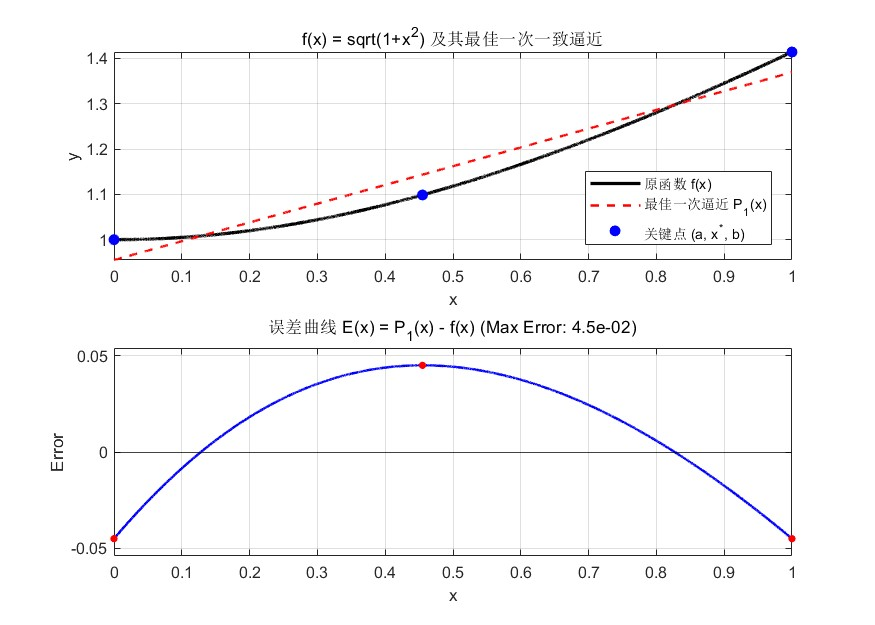
\includegraphics[width=1.0\linewidth]{Best Approximation-sqrt(x^2+1).jpg}
    \label{fig:Best Approximation sqrt(x^2+1)}
    \caption{函数 $\sqrt{x^2+1}$ 的最佳一次一致逼近}
\end{figure}
\begin{example}
    求 $ f(x) = \mathrm{e}^x - 1 $ 在 $[0, 1]$ 上的最佳一致逼近一次多项式.
\end{example}
\begin{solution}
    同样地, $ f(x) = \mathrm{e}^x - 1 $ 在 $[0, 1]$ 上 $ f''(x) = \mathrm{e}^x > 0 $, 为凸函数. 
    首先计算斜率 $ a_1 $: 
    \[ a_1 = \frac{f(1) - f(0)}{1 - 0} = \frac{(\mathrm{e} - 1) - 0}{1} = \mathrm{e} - 1 \approx 1.7183. \]
    确定极值点 $ x^* $, 由 $ f'(x^*) = a_1 $ 得: 
    \[ \mathrm{e}^{x^*} = \mathrm{e} - 1 \iff x^* = \ln(\mathrm{e} - 1) \approx 0.5413. \]
    此时 $ f(x^*) = \mathrm{e}^{x^*} - 1 = (\mathrm{e} - 1) - 1 = \mathrm{e} - 2 $.
    计算截距 $ a_0 $: 
    \[ a_0 = \frac{1}{2} [f(0) + f(x^*) - a_1(0 + x^*)] = \frac{1}{2} [0 + (\mathrm{e} - 2) - (\mathrm{e} - 1)\ln(\mathrm{e} - 1)] \approx -0.1057. \]
    综上, 最佳一次一致逼近多项式为: 
    \[ p_1^*(x) = (\mathrm{e} - 1)x + \frac{1}{2}[\mathrm{e} - 2 - (\mathrm{e} - 1)\ln(\mathrm{e} - 1)] \approx 1.7183 x - 0.1057. \qedhere\]
\end{solution}
我们来看MATLAB编程实验结果: 
\begin{figure}[H]
    \centering
    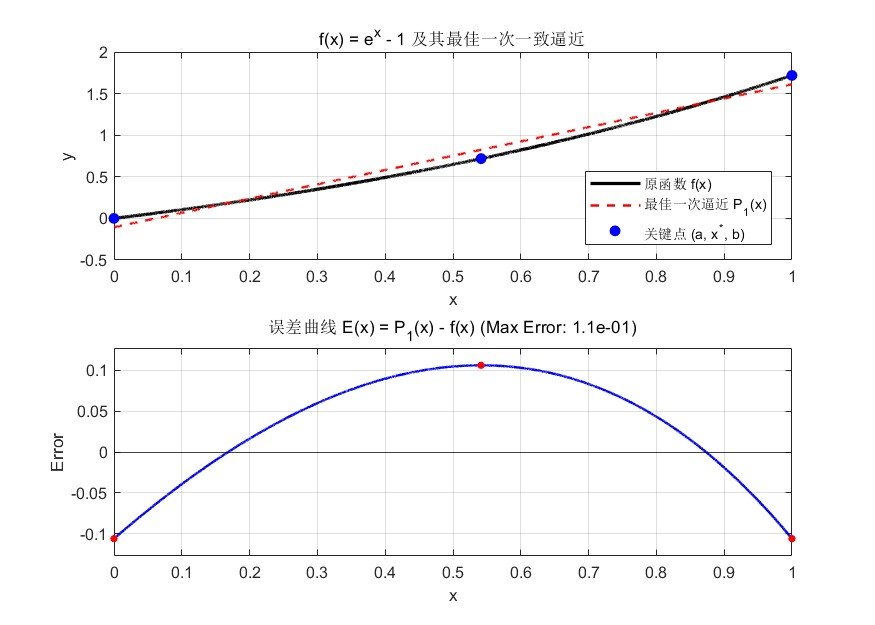
\includegraphics[width=0.85\linewidth]{Best Approximation-e^x-1.jpg}
    \label{fig:Best Approximation exp(x)-1}
    \caption{函数 $\mathrm{e}^x - 1$ 的最佳一次一致逼近及误差曲线}
\end{figure}
可以看到计算最佳一致逼近过程过于复杂, 且对于高次最佳一致逼近多项式没有一般算法. 因此我们会考虑其他范数下的最佳逼近, 或者近似最佳一致逼近.
\section{最佳平方逼近与正交多项式}
\subsection{数学理论基础}
\subsubsection{最佳平方逼近理论}
我们引入如下带权内积
\[ (f, g)_{\rho} := \int_a^b \rho(x) f(x) g(x) \mathrm{d} x. \]
这里的 $ \rho(x) $ 为所谓权函数, 满足以下条件:
\begin{itemize}
    \item[1.] $ \rho(x) \geq 0, \, \forall x \in [a, b]; $
    \item[2.] $ \int_a^b \rho(x) |x|^m \mathrm{d} x < +\infty, \, \forall m \in \mathbb{N} \cup \{0\}; $
    \item[3.] 任给非负连续函数 $ g $, 若 $ \int_a^b \rho(x) g(x) \mathrm{d} x = 0 \implies g \equiv 0 $.
\end{itemize}
由上面带权内积可以诱导出一种 2-范数:
\[ \| f \|_2 := \sqrt{(f, f)} = \left( \int_a^b \rho(x) |f(x)|^2 \right)^{1/2}. \]
令 $ L_{\rho}^2[a, b] := \{ f : [a, b] \rightarrow \mathbb{R} \mid \| f \|_2 < +\infty \} $ 为一线性赋范空间.
设 $ \{\varphi_j\}_{j=0}^n \subset L_{\rho}^2[a, b] $ 为线性无关函数, 记 $ \mathfrak{S} := \operatorname{Span}\{\varphi_0, \cdots, \varphi_n\} $.
\begin{definition}[最佳平方逼近函数]
    设 $ f \in L_{\rho}^2[a, b] $, 若 $ \exists S_n^* \in \mathfrak{S} $ 使得$ \| f - S_n^* \|_2 = \inf_{S \in \mathfrak{S}} \| f - S \|_2 $, 则称 $ S_n^* $ 为 $ f $ 在 $ \mathfrak{S} $ 中的最佳平方逼近函数.
\end{definition}
既然 $ S_n^* \in \mathfrak{S} $, 那么有 $ \{a_j^*\}_{j=0}^n \subset \mathbb{R} $ 使得$ S_n^*(x) = \sum_{j=0}^n a_j^* \varphi_j(x) $. 因此找 $ S_n^* $, 也就是找系数 $ \{a_j^*\}_{j=0}^n $, 使得以下多元函数
\[ I(a_0, \cdots, a_n) = \left\| f - \sum_{j=0}^n a_j \varphi_j \right\|_2^2 = \int \left[ f(x) - \sum_{j=0}^n a_j \varphi_j(x) \right]^2 \rho(x) \mathrm{d} x \]
在 $ \bm{a} = \{a_j^*\}_{j=0}^n $ 达到最小值.

由多元函数求极值的必要条件:
\[ \frac{\partial I}{\partial a_k} \bigg|_{\bm{a}^*} = 0, \quad k = 0, \cdots, n, \quad \bm{a}^* = (a_0^*, \cdots, a_n^*) \]
即
\begin{align}
    0 &= 2 \left( \int_a^b \sum_{j=0}^n a_j \rho(x) \varphi_j(x) \varphi_k(x) \mathrm{d} x - \int_a^b \rho(x) f(x) \varphi_k(x) \mathrm{d} x \right)\\
    &\iff \sum_{j=0}^n a_j (\varphi_j, \varphi_k) = (f, \varphi_k), \quad k = 0, 1, \cdots, n
\end{align}
上述方程组也称为关于 $ (a_0, \cdots, a_n) $ 的\textbf{法方程}. 由高等代数知识知, 上述法方程存在唯一解(即 Gram 矩阵可逆) $ \Longleftrightarrow \{ \varphi_j \}_{j=0}^n $ 线性无关. 因此, 由 $ \{ \varphi_j \}_{j=0}^n $ 为线性无关基函数知, 上述法方程必存在唯一解 $ \bm{a}^* = (a_0^*, \cdots, a_n^*) \in \mathbb{R}^{n+1} $. 记 $ S_n^* = \sum_{j=0}^n a_j^* \varphi_j $. 事实上, 由于前面法方程的成立仅是极值的必要条件, 下面我们还需要验证$ \forall S \in \mathfrak{S}, \| f - S_n^* \|_2^2 \leq \| f - S \|_2^2 $, 这说明 $ S_n^* $ 确实是 $ f $ 在 $ \mathfrak{S} $ 中的最佳平方逼近函数, 且为唯一解. 具体过程我们略去. 

\subsubsection{正交多项式}
但如果我们取 $ \mathfrak{S} = P_n $ 的基函数为 $ \{1, x, \cdots, x^n\} $ 来求最佳平方逼近, 那么我们会发现其 Gram 矩阵为 Hilbert 矩阵, $ n \rightarrow +\infty $ 时其条件数急剧增大. 此时解法方程, 舍入误差会带来很大影响.

为了减少舍入误差影响, 我们一般采用所谓的\textbf{正交多项式} $ \{\varphi_j\}_{j=0}^n $, 即
\[ (\varphi_j, \varphi_k) = A_{jk} = \left\{
\begin{array}{ll}
A_j > 0, & j = k; \\
0, & j \neq k.
\end{array}
\right. \]
这时 Gram 矩阵成为对角矩阵了, 自然法方程也就极易求解了.

因此, 如何得到在带权内积 $ (f, g)_{\rho} = \int_a^b \rho(x) f(x) g(x) \, \mathrm{d} x $ 下的正交多项式成为关键!
\begin{definition}
    设 $ \varphi_n(x) $ 为 $ n $ 次多项式, 如果 $ \{\varphi_j\}_{j=0}^{+\infty} $ 满足
\[ (\varphi_j, \varphi_k) = \int_a^b \rho(x) \varphi_j(x) \varphi_k(x) \, \mathrm{d} x = \left\{
\begin{array}{ll}
A_j \neq 0, & j = k; \\
0, & j \neq k.
\end{array}
\right. \]
则称多项式序列 $ \{\varphi_j\}_{j=0}^{+\infty} $ 在 $[a, b]$ 上带权 $ \rho(x) $ 正交. $ \varphi_n(x) $ 称为 $[a, b]$ 上带权 $ \rho(x) $ 正交的 $ n $ 次多项式.
\end{definition}
下面的定理给出的正交多项式的构造方法. 
\begin{theorem}[Gram-Schmit正交化]
    $ \forall n \geq 0 $, 则存在多项式序列 $ \{\varphi_j\}_{j=0}^n $ 使得 $ \varphi_j $ 为 $ j $ 次多项式, 且
\[ (\varphi_j, \varphi_k) = \delta_{jk} = \left\{
\begin{array}{ll}
1, & j = k; \\
0, & j \neq k.
\end{array}
\right. \]
\end{theorem}
证明是构造性证明, 即求法蕴含在证明过程中. 
\begin{proof}
    设 $ \varphi_0(x) \equiv C $, 欲使 $ (\varphi_0, \varphi_0) = 1 $, 即
    \[ 1 = \int_a^b \rho(x) C^2 \, \mathrm{d} x \iff C = \left( \int_a^b \rho(x) \, \mathrm{d} x \right)^{-1/2}, \]
    (由权函数定义知 $ \int_a^b \rho(x) \cdot 1 \, \mathrm{d} x > 0 $).

    下面我们考虑如何得到 $ \varphi_1 $. 
    
    用待定系数法, 令 $ \psi_1(x) = x + a_{10} \varphi_0(x) $, 使得 $ (\psi_1, \varphi_0) = 0 $, 则
    \[a_{10} = -(x, \varphi_0) = -C \int_a^b \rho(x) x \, \mathrm{d} x. \]
    再令 $ \varphi_1 = \frac{\psi_1}{\| \psi_1 \|_2} $, 便有 $ (\varphi_1, \varphi_1) = 1 $, $ (\varphi_1, \varphi_0) = 0 $.
    一般地, 如果已经求出了 $ \varphi_0, \varphi_1, \cdots, \varphi_{n-1} $, 使得
    \[ (\varphi_j, \varphi_k) = \delta_{jk}, \quad 0 \leq j, k \leq n - 1. \]
    可以令 $ \psi_n(x) = x^n + a_{n,n-1} \varphi_{n-1}(x) + \cdots + a_{n0} \varphi_0(x) $. 欲使 $ (\psi_n, \varphi_j) = 0, \, j = 0, \cdots, n - 1 $, 即有 $ a_{nj} = -(x^n, \varphi_j), \, j = 0, \cdots, n - 1 $. 再令 $ \varphi_n = \frac{\psi_n}{\| \psi_n \|_2} $, 即有 $ (\varphi_n, \varphi_n) = 1 $, $ (\varphi_n, \varphi_j) = 0, \, 0 \leq j \leq n - 1 $. 这样我们便得到了正交多项式序列 $ \{\varphi_j\}_{j=0}^n $. 
\end{proof}
将上述步骤整理成伪代码, 即
\begin{algorithm}[H]
\caption{Gram-Schmidt 正交化构造规范正交多项式}
\label{alg:gram_schmidt_poly}
\begin{algorithmic}[1]
\REQUIRE 最高阶数 $n$, 区间 $[a, b]$, 权函数 $\rho(x)$
\ENSURE 规范正交多项式序列 $\{\varphi_0, \varphi_1, \dots, \varphi_n\}$

\STATE \textbf{Step 1: 初始化 (构造 $\varphi_0$)}
\STATE 计算 $0$ 次基函数的模长: 
\[ N_0 \leftarrow \sqrt{\int_a^b \rho(x) \cdot 1^2 \, \mathrm{d}x} \]
\STATE 归一化得到首个多项式: 
\[ \varphi_0(x) \leftarrow \frac{1}{N_0} \]

\STATE \textbf{Step 2: 迭代构造 (构造 $\varphi_1$ 到 $\varphi_n$)}
\FOR{$k = 1$ to $n$}
    \STATE \textbf{2.1 正交化 (构造辅助多项式 $\psi_k$)}
    \STATE 设 $\psi_k(x)$ 的形式为 $x^k + \sum_{j=0}^{k-1} a_{kj} \varphi_j(x)$
    \FOR{$j = 0$ to $k-1$}
        \STATE 计算投影系数(内积): 
        \[ a_{kj} \leftarrow - (x^k, \varphi_j) = - \int_a^b \rho(x) x^k \varphi_j(x) \, \mathrm{d}x \]
    \ENDFOR
    \STATE 组装正交多项式(尚未归一化): 
    \[ \psi_k(x) \leftarrow x^k + \sum_{j=0}^{k-1} a_{kj} \varphi_j(x) \]

    \STATE \textbf{2.2 归一化}
    \STATE 计算模长: 
    \[ \|\psi_k\|_2 \leftarrow \sqrt{\int_a^b \rho(x) [\psi_k(x)]^2 \, \mathrm{d}x} \]
    \STATE 得到第 $k$ 个规范正交多项式: 
    \[ \varphi_k(x) \leftarrow \frac{\psi_k(x)}{\|\psi_k\|_2} \]
\ENDFOR

\RETURN $\{\varphi_0, \varphi_1, \dots, \varphi_n\}$
\end{algorithmic}
\end{algorithm}
设 $ f \in L_{\rho}^2[a, b] = \left\{ f : [a, b] \rightarrow \mathbb{R} \colon \| f \|_2^2 = \int_a^b \rho(x) |f(x)|^2 \, \mathrm{d} x < +\infty \right\},\mathfrak{S} = \text{span}\{\varphi_0, \cdots, \varphi_n\} $, 且设 $ (\varphi_i, \varphi_j) = \left\{
\begin{array}{ll}
0, & i \neq j \\
A_i > 0, & i = j
\end{array}
\right. $.
为求 $ f $ 在 $ \mathfrak{S} $ 上的最佳平方逼近 $ S_n^* $ 使得 $ \| f - S_n^* \|_2^2 = \inf_{S \in \mathfrak{S}} \| f - S \|_2^2 $, 设 $ S_n^* = \sum_{j=0}^n \alpha_j^* \varphi_j(x) $, 由前面最佳平方逼近理论, 及基函数 $ \{\varphi_j\} $ 的正交性, 我们有
\begin{equation}
    \alpha_k^* (\varphi_k, \varphi_k) = (f, \varphi_k) \implies \alpha_k^* = \frac{(f, \varphi_k)}{(\varphi_k, \varphi_k)}.
\end{equation}
前面已经证明过 $ S_n^* $ 确实为 $ f $ 在 $ \mathfrak{S} $ 上的最佳平方逼近.

令误差 $ \delta_n = f - S_n^* $, 由 $ (f, \varphi_k) = \alpha_k^* (\varphi_k, \varphi_k) \iff (f, S_n^*) = (S_n^*, S_n^*) $
\[ \iff \| \delta_n \|_2^2 = (f, f) - (S_n^*, S_n^*) - 2(f, S_n^*) = (f, f) - (S_n^*, S_n^*) \]

\begin{definition}
    $ \forall f \in L_{\rho}[a, b] $, $ \{\varphi_j\}_{j \geq 0} $ 为正交函数组(不一定是多项式), 称
    \begin{equation}
        \alpha_j = \frac{(f, \varphi_j)}{(\varphi_j, \varphi_j)} = \frac{1}{(\varphi_j, \varphi_j)} \int_a^b \rho(x) f(x) \varphi_j(x) \, \mathrm{d} x, \, j = 0, 1, \cdots
    \end{equation}
    为 $ f $ 在正交函数组 $ \{\varphi_j\}_{j \geq 0} $ 下的广义 Fourier 系数, 相应地称级数
    \[ \sum_{j=0}^{+\infty} \alpha_j \varphi_j(x) \]
    为 $ f $ 的广义 Fourier 级数.
\end{definition}
从上面最佳平方逼近的定义可以看出, $ f $ 的最佳平方逼近就是它的广义 Fourier 级数前 $ n+1 $ 项的部分和. 最后我们来看它的收敛性. 
\begin{theorem}[$ L^2 $ 范数下的收敛性]
    设 $ f \in C[a, b] $, $ S_n^* $ 为 $ f $ 在 $ \mathfrak{S} = \text{span}\{\varphi_0, \cdots, \varphi_n\} $ 上的最佳平方逼近多项式, 则有
\[ \lim_{n \rightarrow +\infty} \| f - S_n^* \|_2 = 0. \]
\end{theorem}

\subsection{Chebyshev 多项式逼近}
在区间 $[-1, 1]$ 上, 权函数为 $\rho(x) = \frac{1}{\sqrt{1-x^2}}$. 此时正交多项式系为 Chebyshev 多项式 $\{T_j\}_{j=0}^n$. 
设 $f \in L^2_{\rho}[-1, 1]$, 其在 $S = \text{span}\{T_j\}_{j=0}^n$ 上的最佳平方逼近为: 
\[ S_n^*(x) = \sum_{j=0}^n \alpha_j T_j(x), \]
其中系数 $\alpha_j$ 计算公式为: 
\[ \alpha_j = \frac{(f, T_j)}{(T_j, T_j)}, \quad (T_j, T_j) = \begin{cases} \pi, & j=0; \\ \pi/2, & j \ne 0. \end{cases} \]

\begin{example}
    设 $\rho(x) = \frac{1}{\sqrt{1-x^2}}$, 求 $f(x) = \cos x$ 在 $[-1, 1]$ 上的最佳平方逼近多项式($n=3$). 
\end{example}
\begin{solution}
    计算内积: 
    \begin{align*}
        (f, T_0) &= \int_{-1}^1 \frac{\cos x}{\sqrt{1-x^2}} \, \mathrm{d} x \approx 2.404,\quad (f, T_1) = 0;\\
        (f, T_2) &= \int_{-1}^1 \frac{(2x^2-1)\cos x}{\sqrt{1-x^2}} \, \mathrm{d} x \approx -0.3610,\quad (f, T_3) = 0.
    \end{align*}
    于是最佳平方逼近多项式为: 
    \[ S_3^*(x) = \frac{2.404}{\pi} T_0(x) + \frac{-0.3610}{\pi/2} T_2(x) \approx -0.460 x^2 + 0.995, \]
    误差估计: $\|f - S_3^*\|_\infty \approx 5.00 \times 10^{-3}$. 
\end{solution}
我们来看MATLAB编程实验结果: 
\begin{figure}[H]
    \centering
    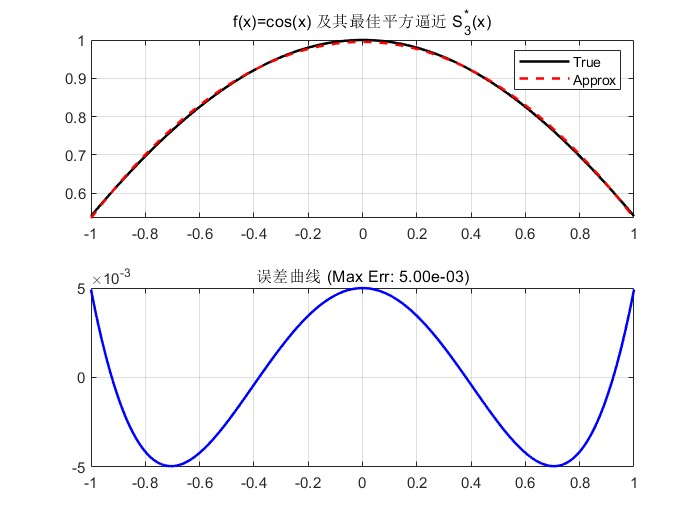
\includegraphics[width=0.9\linewidth]{Best Square Approximation-cos(x).jpg}
    \label{fig:Best Square Approximation-cos(x)}
    \caption{函数 $\cos(x)$ 的最佳平方三次逼近及误差曲线}
\end{figure}
\begin{example}
    设 $\rho(x) = \frac{1}{\sqrt{1-x^2}}$, 求 $f(x) = \ln(1+x^2)$ 在 $[-1, 1]$ 上的最佳平方逼近多项式($n=3$). 
\end{example}
\begin{solution}
    计算内积: 
    \begin{align*}
        (f, T_0) &= \int_{-1}^1 \frac{\ln(1+x^2)}{\sqrt{1-x^2}} \, \mathrm{d} x \approx 1.1816,\quad (f, T_1) = 0;\\
        (f, T_2) &= \int_{-1}^1 \frac{(2x^2-1)\ln(1+x^2)}{\sqrt{1-x^2}} \, \mathrm{d} x \approx -0.5390,\quad (f, T_3) = 0.
    \end{align*}
    (注: 由于 $f(x)$ 为偶函数, 故与奇次多项式 $T_1, T_3$ 的内积为 0).

    于是最佳平方逼近多项式为: 
    \[ S_3^*(x) = \frac{1.1816}{\pi} T_0(x) + \frac{-0.5390}{\pi/2} T_2(x) \approx 0.3761 - 0.3431(2x^2-1) \approx -0.6862 x^2 + 0.7192, \]
    误差估计: $\|f - S_3^*\|_\infty \approx 2.60 \times 10^{-2}$. 
\end{solution}
我们来看MATLAB编程实验结果: 
\begin{figure}[H]
    \centering
    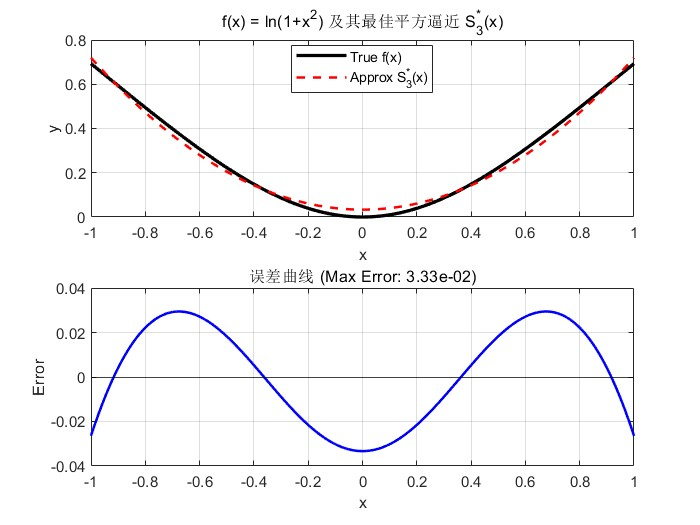
\includegraphics[width=0.9\linewidth]{Best Square Approximation-ln(1+x^2).jpg}
    \label{fig:Best Square Approximation-ln(1+x^2)}
    \caption{函数 $\ln(1+x^2)$ 的最佳平方三次逼近及误差曲线}
\end{figure}

\subsection{Lagrange 插值余项与 Chebyshev 节点}
Lagrange 插值多项式 $L_n(x)$ 的余项为: 
\[ R_n(x) = f(x) - L_n(x) = \frac{f^{(n+1)}(\xi)}{(n+1)!} \omega_{n+1}(x) \]
其中 $\omega_{n+1}(x) = \prod_{j=0}^n (x - x_j)$. 
误差上界取决于 $\|\omega_{n+1}\|_\infty$. 
为了使误差最小, 应选择节点使得 $\|\omega_{n+1}\|_\infty$ 最小. 
已知首项系数为 1 的 $n+1$ 次多项式中, Chebyshev 多项式 $\frac{1}{2^n} T_{n+1}(x)$ 具有最小的 $\infty$-范数. 
因此, 最佳插值节点应选为 $T_{n+1}(x)$ 的零点: 
\[ x_k = \cos \frac{2k+1}{2(n+1)}\pi, \quad k=0, 1, \dots, n \]
此时误差界为: 
\[ \|R_n\|_\infty \le \frac{M_{n+1}}{(n+1)! 2^n} \]

\begin{example}
    以 $f(x) = \cos x$ 为例, 比较 Lagrange 插值(使用 Chebyshev 节点)与最佳一致逼近. 
\end{example}
\begin{solution}
    取 $n=3$, 节点为 $T_4(x)$ 的零点: $x_j = \pm \sqrt{\frac{2 \pm \sqrt{2}}{4}}$. 
    计算得到的插值多项式为: 
    \[ L_3(x) \approx -0.45953 x^2 + 0.99496, \]
    这与之前的最佳平方逼近 $S_3^*(x)$ 非常接近. 
    误差 $\|f - L_3\|_\infty \approx 5.0374 \times 10^{-3}$. 
\end{solution}
下面是Matlab实验结果：
\begin{figure}[H]
    \centering
    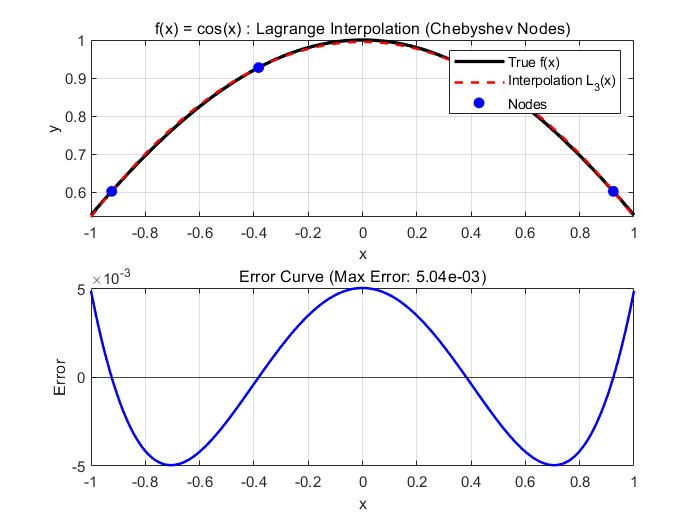
\includegraphics[width=0.9\linewidth]{Lagrange Chebyshev f(x)=cos(x).jpg}
    \label{fig:Lagrange Chebyshev f(x)=cos(x)}
    \caption{函数 $\cos(x)$ 的Lagrange插值(使用Chebyshev误差节点)及误差曲线}
\end{figure}
\begin{example}
    以 $f(x) = \ln(1+x^2)$ 为例, 比较 Lagrange 插值(使用 Chebyshev 节点)与最佳一致逼近. 
\end{example}
\begin{solution}
    取 $n=3$, 节点为 $T_4(x)$ 的零点: 
    \[ x_k = \cos\left(\frac{2k-1}{8}\pi\right), \quad k=1, 2, 3, 4. \]
    具体数值为 $x_1, x_4 \approx \pm 0.9239$, $x_2, x_3 \approx \pm 0.3827$.
    
    计算得到的插值多项式为: 
    \[ L_3(x) \approx 0.6794 x^2 + 0.0372, \]
    这与之前的最佳平方逼近 $S_3^*(x)$ 非常接近. 
    误差 $\|f - L_3\|_\infty \approx 0.0372$ (在 $x=0$ 处, $f(0)=0, L_3(0)=0.0372$).
\end{solution}
\begin{figure}[H]
    \centering
    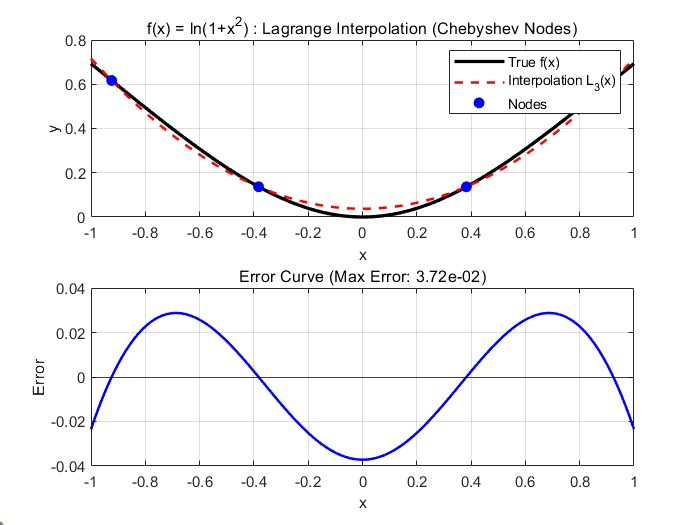
\includegraphics[width=0.9\linewidth]{Lagrange Chebyshev f(x)=ln(1+x^2).jpg}
    \label{fig:Lagrange Chebyshev f(x)=ln(1+x^2)}
    \caption{函数 $\ln(1+x^2)$ 的Lagrange插值(使用Chebyshev误差节点)及误差曲线}
\end{figure}
\section{Padé逼近 (Padé Approximation)}
前面考虑的都是用光滑函数(多项式)来逼近连续函数, 显然用多项式来逼近函数有不少优点, 如: 
\begin{itemize}
    \item[1.] 闭区间上可以用多项式来任意逼近连续函数; 
    \item[2.] 多项式易于计算(求值、求导以及积分等). 
\end{itemize}
但是我们也看到多项式逼近有时会产生伪振荡, 且若 $ f $ 本身有奇点时用多项式来逼近可能不是很好选择. 而用有理函数逼近有时效果更好, 可以克服这些缺点. 
\subsection{数学理论基础}
\begin{definition}[Pad\'e逼近]
    若对 $ f \in C^{(N+1)}[-a, a], N = n + m $, 有理函数
    \[ R_{nm}(x) = \frac{P_n(x)}{Q_m(x)} = \sum_{k=0}^{n} a_k x^k / \sum_{k=0}^{m} b_k x^k \]
    满足
    \[ R_{nm}^{(k)}(0) = f^{(k)}(0) \equiv P_N^{(k)}(0), \quad k = 0, 1, \cdots, N \]
    则称 $ R_{nm}(x) $ 为 $ f(x) $ 在 $ x = 0 $ 处的 $ (n, m) $ 阶 Pad\'e 逼近, 记为 $ R(n, m) $. 
\end{definition}
由上述定义可知 $ \left( P_N(x) - R_{nm}(x) \right)^{(k)} \big|_{x=0} = 0, \, k = 0, 1, \cdots, N $. 
这样设 $ g(x) $ 为任一光滑函数, 那么按二项式展开即得, 
\[ \left[ g(x) \cdot \left( P_N(x) - R_{nm}(x) \right) \right]^{(k)} \big|_{x=0} = 0. \]

因此我们取 $ g(x) = Q_m(x) $, 令
\[ h(x) = Q_m(x) \cdot (P_N - R_{nm})(x) = Q_m P_N - P_n \] 为一多项式, 有
\[ h^{(k)}(0) = 0, \quad k = 0, 1, \cdots, N \]
即\begin{align*}
    0 &= (Q_m P_N - P_n)^{(k)}(0) = \sum_{j=0}^{k} \binom{k}{j} P_N^{(j)}(0) Q_m^{(k-j)}(0) - k! a_k
    \\&= k! \left[ \sum_{j=0}^{k} c_j b_{k-j} - a_k \right], \quad k = 0, 1, \cdots, N.
\end{align*}
当 $ k - j > m $ 时, $ b_{k-j} \equiv 0 $; $ k > n $ 时, $ a_k \equiv 0 $. 因此有(注意 $ b_0 = 1 $)
\begin{align}
    0 & = c_k + \sum_{j=(k-m,0)+}^{k-1} c_j b_{k-j}, \quad k = n+1, \cdots, n+m; \\
    \label{eq:Pade approx-coefficients 2}a_k & = c_k + \sum_{j=(k-m,0)+}^{k-1} c_j b_{k-j}, \quad k = 0, 1, \cdots, n.
\end{align}
令 \[\bm{H} := \begin{pmatrix}
c_n & c_{n-1} & \cdots & c_{n-m+1} \\
c_{n+1} & c_n & \cdots & c_{n-m+2} \\
\vdots & \vdots & & \vdots \\
c_{n+m-1} & c_{n+m-2} & \cdots & c_n
\end{pmatrix}, \, \bm{b} = \begin{pmatrix}
b_1 \\
\vdots \\
b_m
\end{pmatrix}, \, \bm{c} = -\begin{pmatrix}
c_{n+1} \\
\vdots \\
c_{n+m}
\end{pmatrix}.\]
先解方程组 $ \bm{Hb} = \bm{c} $ 得 $ \bm{b} $, 然后再由\eqref{eq:Pade approx-coefficients 2}式计算得 $ \{a_k\}_{k=0}^n $. 

上述步骤可以总结为下面的伪代码: 
\begin{algorithm}[H]
\caption{Padé 逼近系数求解算法 ([L/M] 阶)}
\begin{algorithmic}[1]
\REQUIRE Taylor系数向量 $\mathbf{c} = [c_0, \dots, c_{L+M}]$, 阶数 $L, M$
\ENSURE 分子系数 $\mathbf{a}$, 分母系数 $\mathbf{b}$

\STATE \textbf{Step 1: 构建 Toeplitz 系统}
\STATE 构造矩阵 $\mathbf{H} \in \mathbb{R}^{M \times M}$, 其中 $H_{ij} = c_{L-M+i+j-1}$ (若下标越界则为0). 
\STATE 构造右端向量 $\mathbf{y} = [-c_{L+1}, \dots, -c_{L+M}]^T$. 

\STATE \textbf{Step 2: 求解分母系数}
\STATE 解方程 $\mathbf{H} \tilde{\mathbf{b}} = \mathbf{y}$ 得到 $\tilde{\mathbf{b}} = [b_M, \dots, b_1]^T$. 
\STATE 令 $b_0 = 1$, 完整分母系数为 $\mathbf{b} = [1, b_1, \dots, b_M]$. 

\STATE \textbf{Step 3: 计算分子系数}
\FOR{$k = 0$ to $L$}
    \STATE $a_k = \sum_{j=0}^{\min(k,M)} c_{k-j} b_j$
\ENDFOR

\RETURN $\mathbf{a}, \mathbf{b}$
\end{algorithmic}
\end{algorithm}
\subsection{编程实验: 几个初等函数的Padé逼近计算与图像对比}
下面我们采用Padé逼近计算几个初等函数的有理逼近式子:
\newpage
\begin{table}[H]
    \centering
    \caption{函数 $\mathrm{e}^x$ 在 $x=0$ 处的 Padé 逼近公式}
    \label{tab:pade_ex}
    \renewcommand{\arraystretch}{1.5}
    \begin{tabular}{c|c}
        \toprule
        \textbf{阶数 [L/M]} & \textbf{Padé 逼近式 $R(x)$} \\ \midrule
        $[1/0]$ & $1+x$ \\ 
        $[0/1]$ & $\dfrac{1}{1-x}$ \\ 
        $[1/1]$ & $\dfrac{2+x}{2-x}$ \\ 
        $[1/2]$ & $\dfrac{6+2x}{6-4x+x^2}$ \\ 
        $[2/1]$ & $\dfrac{6+4x+x^2}{6-2x}$ \\ 
        $[2/2]$ & $\dfrac{12+6x+x^2}{12-6x+x^2}$ \\ \bottomrule
    \end{tabular}
\end{table}

\begin{figure}[H]
    \centering
    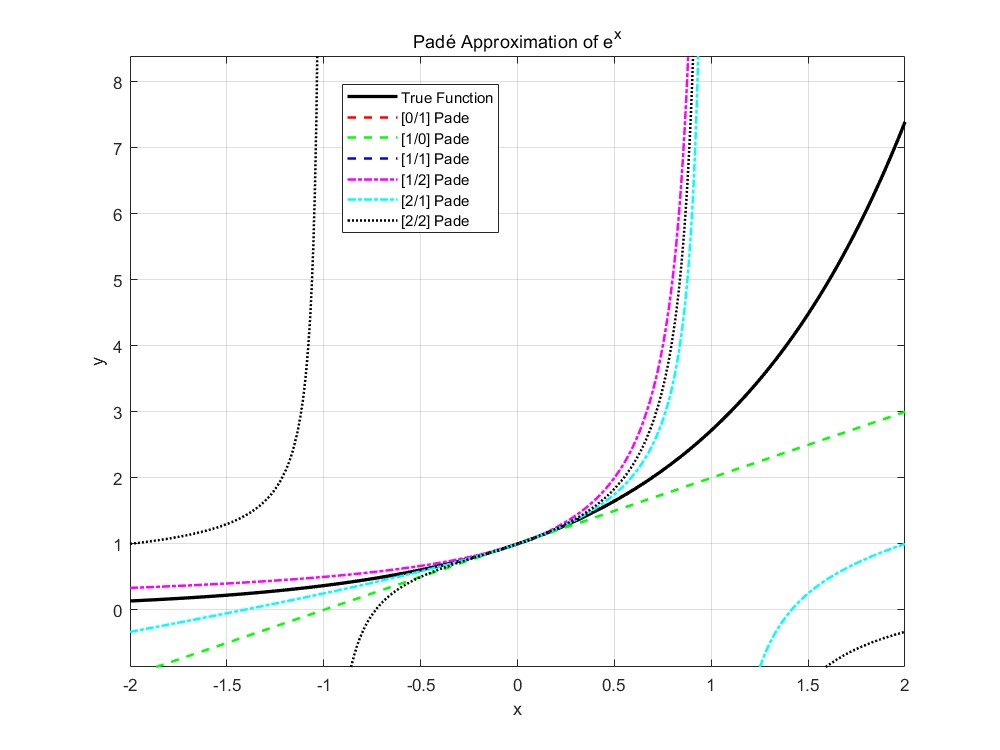
\includegraphics[width=1.0\linewidth]{Pade Approx e^x.jpg}
    \label{fig:Pade Approx e^x}
    \caption{函数 $\mathrm{e}^x$ 的 Padé 逼近式}
\end{figure}
\begin{table}[H]
    \centering
    \caption{函数 $\ln(1+x)$ 在 $x=0$ 处的 Padé 逼近公式}
    \label{tab:pade_ln}
    \renewcommand{\arraystretch}{1.5}
    \begin{tabular}{c|c}
        \toprule
        \textbf{阶数 [L/M]} & \textbf{Padé 逼近式 $R(x)$} \\ \midrule
        $[1/0]$ & $x$ \\ 
        $[0/1]$ & $\dfrac{x}{1+x}$ \\ 
        $[1/1]$ & $\dfrac{2x}{2+x}$ \\ 
        $[1/2]$ & $\dfrac{12x}{12+6x-x^2}$ \\ 
        $[2/1]$ & $\dfrac{x(6+x)}{6+4x}$ \\ 
        $[2/2]$ & $\dfrac{6x+3x^2}{6+6x+x^2}$ \\ \bottomrule
    \end{tabular}
\end{table}

\begin{figure}[H]
    \centering
    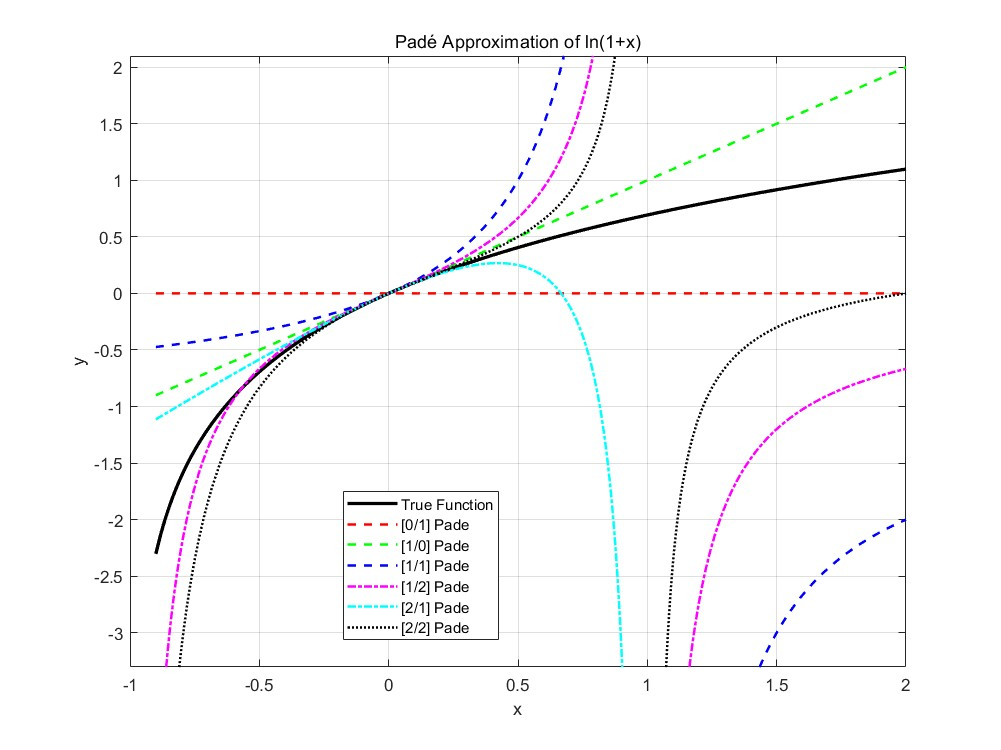
\includegraphics[width=1.0\linewidth]{Pade Approx ln(1+x).jpg}
    \label{fig:Pade Approx ln(1+x)}
    \caption{函数 $\ln(1+x)$ 的 Padé 逼近式}
\end{figure}
\begin{table}[H]
    \centering
    \caption{函数 $\tan(x)$ 在 $x=0$ 处的 Padé 逼近公式}
    \label{tab:pade_tan}
    \renewcommand{\arraystretch}{1.5}
    \begin{tabular}{c|c}
        \toprule
        \textbf{阶数 [L/M]} & \textbf{Padé 逼近式 $R(x)$} \\ \midrule
        $[1/0]$ & $x$ \\ 
        $[0/1]$ & $x$ (退化) \\ 
        $[1/1]$ & $x$ (退化) \\ 
        $[1/2]$ & $\dfrac{3x}{3-x^2}$ \\ 
        $[2/1]$ & $\dfrac{3x}{3-x^2}$ (退化为 [1/2]) \\ 
        $[2/2]$ & $\dfrac{3x}{3-x^2}$ (退化为 [1/2]) \\ \bottomrule
    \end{tabular}
\end{table}

\begin{figure}[H]
    \centering
    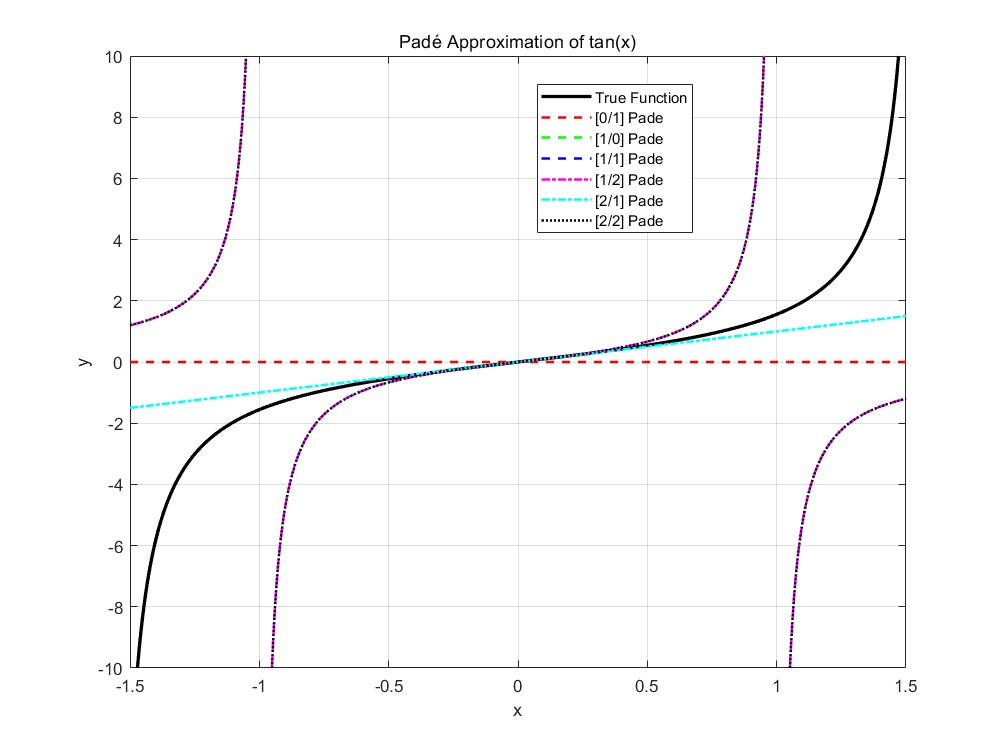
\includegraphics[width=1.0\linewidth]{Pade Approx tan(x).jpg}
    \label{fig:Pade Approx tan x}
    \caption{函数 $\tan x$ 的 Padé 逼近式}
\end{figure}
\begin{table}[H]
    \centering
    \caption{函数 $\sin(x)$ 在 $x=0$ 处的 Padé 逼近公式}
    \label{tab:pade_sin}
    \renewcommand{\arraystretch}{1.5}
    \begin{tabular}{c|c}
        \toprule
        \textbf{阶数 [L/M]} & \textbf{Padé 逼近式 $R(x)$} \\ \midrule
        $[1/0]$ & $x$ \\ 
        $[0/1]$ & $x$ (退化) \\ 
        $[1/1]$ & $x$ (退化) \\ 
        $[1/2]$ & $\dfrac{6x}{6+x^2}$ \\ 
        $[2/1]$ & $\dfrac{6x-x^3}{6}$ (Taylor) \\ 
        $[2/2]$ & $\dfrac{6x}{6+x^2}$ (退化为 [1/2]) \\ \bottomrule
    \end{tabular}
\end{table}

\begin{figure}[H]
    \centering
    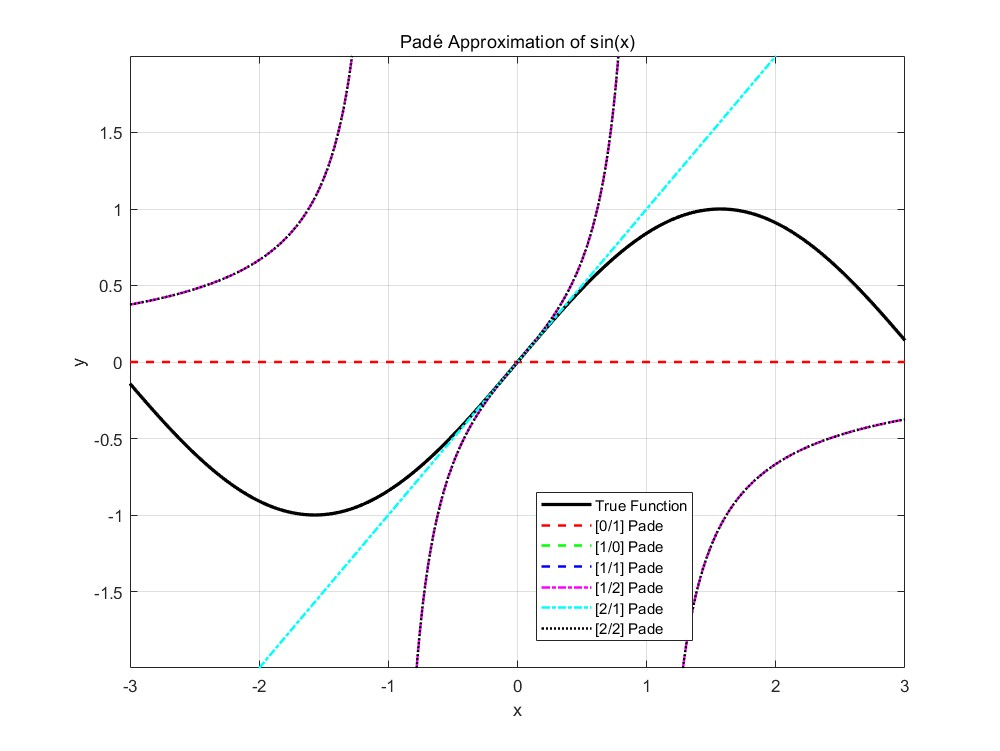
\includegraphics[width=1.0\linewidth]{Pade Approx sin(x).jpg}
    \label{fig:Pade Approx sin x}
    \caption{函数 $\sin x$ 的 Padé 逼近式}
\end{figure}
\begin{table}[H]
    \centering
    \caption{函数 $\cos(x)$ 在 $x=0$ 处的 Padé 逼近公式}
    \label{tab:pade_cos}
    \renewcommand{\arraystretch}{1.5}
    \begin{tabular}{c|c}
        \toprule
        \textbf{阶数 [L/M]} & \textbf{Padé 逼近式 $R(x)$} \\ \midrule
        $[1/0]$ & $1$ \\ 
        $[0/1]$ & $1$ (退化) \\ 
        $[1/1]$ & $1$ (退化) \\ 
        $[1/2]$ & $\dfrac{2}{2+x^2}$ \\ 
        $[2/1]$ & $1 - \dfrac{1}{2}x^2$ (Taylor) \\ 
        $[2/2]$ & $\dfrac{12-5x^2}{12+x^2}$ \\ \bottomrule
    \end{tabular}
\end{table}

\begin{figure}[H]
    \centering
    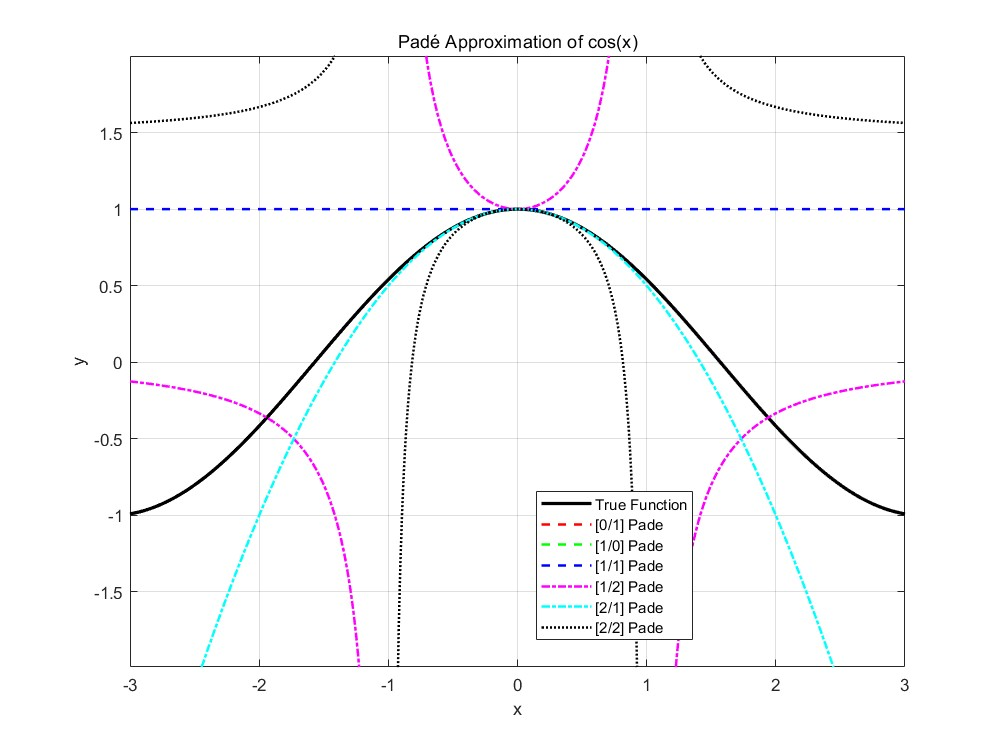
\includegraphics[width=1.0\linewidth]{Pade Approx cos(x).jpg}
    \label{fig:Pade Approx cos x}
    \caption{函数 $\cos x$ 的 Padé 逼近式}
\end{figure}
基于上述对 $\mathrm{e}^x, \ln(1+x), \tan x$ 等函数的数值实验, 我们可以从收敛速度、奇点处理及渐近行为三个维度对 Padé 逼近的性能进行深入分析. 
\subsection{逼近性能分析}
\subsubsection{逼近阶数与局部收敛速度}
Padé 逼近 $[L/M]$ 的定义决定了其在展开点(此处为 $x=0$)附近的误差阶为: 
\begin{equation}
    E(x) = f(x) - R_{L,M}(x) = O(x^{L+M+1})
\end{equation}
这表明, 逼近的总阶数 $N = L+M$ 决定了局部收敛的速度. 

观察表 \ref{tab:pade_ex} 中的 $\mathrm{e}^x$, $[1/1]$ 阶逼近(总阶数2)的误差为 $O(x^3)$, 与 $[2/0]$ 阶Taylor展开相同. 然而, 数值结果显示, 在相同总阶数下, 对角线型 Padé 逼近($L=M$)通常比单纯的Taylor展开($M=0$)具有更小的系数常数, 从而在 $x$ 稍大时提供更高的精度. 因此, 随着 $L$ 和 $M$ 的增加, 逼近函数在原点附近的“平坦”区域迅速变宽, 收敛速度呈幂律增长. 

\subsubsection{奇点模拟与有效范围的扩展}
这是 Padé 逼近相对于多项式逼近(Taylor展开)最显著的优势. 多项式函数在复平面上是整函数, 无法模拟有限处的奇点(极点), 导致其收敛半径受限于距离原点最近的奇点. 而有理函数可以通过分母的零点来模拟原函数的极点. 

就拿$\tan x$来说. $\tan x$ 在 $x = \pm \pi/2 \approx \pm 1.57$ 处存在一阶极点, 如果使用Taylor级数, 无论阶数多高, 其收敛半径严格限制在 $|x| < \pi/2$. 在 $x=1.5$ 处, 低阶Taylor级数误差极大. 而使用Padé逼近, 我们观察表 \ref{tab:pade_tan} 中的 $[1/2]$ 阶逼近 $R(x) = \frac{3x}{3-x^2}$. 其分母 $3-x^2$ 的零点为 $x = \pm \sqrt{3} \approx \pm 1.732$. 虽然这与真实的 $\pi/2$ 略有偏差, 但它成功构造了一个“人造极点”, 使得逼近曲线能够跟随 $\tan x$ 趋向无穷大. 这使得有效逼近范围突破了 $\pi/2$ 的限制(在极点外侧也能通过解析延拓逼近).

同样分析$\ln(1+x)$. $\ln(1+x)$ 在 $x=-1$ 处有对数奇点. Taylor级数在 $x > 1$ 时发散. 而 $[1/1]$ 阶 Padé 逼近 $\frac{2x}{2+x}$ 在 $x \to \infty$ 时趋于常数 2, 虽然 $\ln(1+x)$ 趋于无穷, 但相比于Taylor多项式趋于 $\pm \infty$ 的发散速度, Padé 逼近在 $x$ 较大的正半轴上往往能维持更长时间的数值稳定性. 

\subsubsection{无穷远处的渐近行为}
对于物理建模, 函数在 $x \to \infty$ 处的行为至关重要. 
\begin{itemize}
    \item \textbf{多项式缺陷: } $\lim_{x\to\infty} P_n(x) = \infty$, 这对于有界函数(如 $\sin x, \cos x$)或衰减函数是完全错误的. 
    \item \textbf{Padé 优势: } 对于 $[L/M]$ 阶 Padé 逼近: 
    \begin{equation}
        \lim_{x\to\infty} R_{L,M}(x) \approx \lim_{x\to\infty} \frac{a_L x^L}{b_M x^M} = \begin{cases} 
        0, & L < M \\
        \text{const}, & L = M \\
        \infty, & L > M
        \end{cases}
    \end{equation}
    因此, 对于 $\sin x$ 或 $\mathrm{e}^{-x}$ 这类有界或衰减函数, 选择 $L \le M$ 的 Padé 逼近(如表 \ref{tab:pade_sin} 中的 $[1/2]$ 阶 $\frac{6x}{6+x^2}$)能保证数值解在无穷远处不发散, 具有更好的全局稳定性. 
\end{itemize}

\subsubsection{总结}
综上所述, Padé 逼近通过引入分母多项式, 不仅继承了Taylor展开在原点的高精度特性, 更通过模拟极点结构, 显著扩大了收敛域. 在处理具有奇点、渐近线或大范围变化的函数拟合问题时, Padé 逼近是比多项式逼近更优的选择. 

\section{实验总结与分析}
本文基于 MATLAB 平台, 结合数值分析教材中的理论框架, 系统研究了函数逼近与数值拟合的多种核心算法. 通过对 $f(x) = \cos x, \ln(1+x^2), \mathrm{e}^x, \sqrt{1+x^2}$ 等函数的数值实验, 得出以下结论：
\begin{enumerate}
    \item 计算最佳一致逼近过程过于复杂, 且对于高次最佳一致逼近多项式没有一般算法. 
    \item 实验验证了在加权 $L_2$ 空间(权函数 $\rho(x) = \frac{1}{\sqrt{1-x^2}}$)中, 利用 Chebyshev 多项式构造最佳平方逼近的优越性. 
\begin{itemize}
    \item \textbf{系数衰减性：} 对于光滑函数(如 $\cos x$), Chebyshev级数系数 $|c_k|$ 随 $k$ 迅速衰减(如 $c_0 \approx 2.404, c_2 \approx -0.361, c_4 \approx 0$). 实验显示, 仅取前几项($n=3$)即可获得极高的精度(误差量级 $10^{-3}$). 
    \item \textbf{数值稳定性：} 利用正交性计算系数避免了直接求解病态法方程组, 保证了高阶逼近时的数值稳定性. 
\end{itemize}
    \item 针对存在奇点或渐近行为特殊的函数(如 $\ln(1+x^2)$), Padé 逼近展现了独特的优势. 实验表明, Padé 逼近通过分母多项式的零点模拟函数的极点结构, 比单纯的多项式逼近能获得更大的收敛半径. 
\end{enumerate}

\section{不足与改进方向}
尽管本次实验涵盖了主要的逼近方法, 但在实验广度和深度上仍存在以下不足, 可在后续研究中改进：
\subsection{Runge 现象的数值探究}
\begin{itemize}
    \item \textbf{不足：} 本次实验主要关注了 $\cos x$ 和 $\ln(1+x^2)$ 等性质较好的函数, 对于$f(x) = \frac{1}{1+25x^2}$ 在等距节点插值下会出现严重的 Runge 现象(两端振荡发散), 而使用 Chebyshev 节点可以消除此现象. 我们未对 Runge 现象进行具体的数值复现和对比绘图. 
    \item \textbf{改进：} 增加针对 $f(x) = \frac{1}{1+25x^2}$ 的对比实验, 分别绘制高阶(如 $n=10, 14$)等距插值和Chebyshev插值的图像, 直观展示 Chebyshev 节点对插值稳定性的巨大提升. 
\end{itemize}

\subsection{Remez 算法的完整实现}
\begin{itemize}
    \item \textbf{不足：} 本文虽然通过Chebyshev截断近似了最佳一致逼近, 但未实现求解精确最佳一致逼近多项式的 Remez 交换算法. 对于精度要求极高的应用, 近似解可能不够. 
    \item \textbf{改进：} 编写完整的 Remez 算法程序, 通过迭代寻找偏差点组, 求得精确的 Minimax 解, 并量化其与Chebyshev插值解在最大误差上的微小差异. 
\end{itemize}

\subsection{算法实现的通用性}
\begin{itemize}
    \item \textbf{不足：} 目前的代码针对特定函数采用了硬编码的积分计算或解析解. 
    \item \textbf{改进：} 开发通用的逼近工具箱, 利用 MATLAB 的符号计算或自适应积分, 实现对任意用户输入函数的自动逼近与绘图. 
\end{itemize}

\section{个人想法}
    下学期开有数值分析及数值分析实践课, 所以借此机会预习一部分, 这里是自己感兴趣的函数逼近的内容. 由于时间紧迫, 有常微分方程期末考试, 所以结课论文教得晚了. 后面自己还需要复习概率论, 所以借助了AI提高效率, 自己主要负责理论部分的推导和例子的选取, 代码部分一部分是自己写的, 一部分是自己修改. 在MATLAB中都运行通过了. 最后的实验改进部分是借助于AI写的. 
\begin{thebibliography}{99}
\bibitem{burden} Burden R L, Faires J D. Numerical Analysis [M]. 10th ed. Cengage Learning, 2015.
\bibitem{li} 李庆扬, 王能超, 易大义. 数值分析 (第5版) [M]. 北京: 清华大学出版社, 2008.
\bibitem{trefethen} Trefethen L N. Approximation Theory and Approximation Practice [M]. SIAM, 2013.
\bibitem{matlab} The MathWorks, Inc. MATLAB Documentation [EB/OL]. 2023.
\bibitem{powell} Powell M J D. Approximation Theory and Methods [M]. Cambridge University Press, 1981. 
\bibitem{baker} Baker G A, Graves-Morris P. Padé Approximants [M]. Cambridge University Press, 1996. 
\bibitem{matlab} The MathWorks, Inc. MATLAB Documentation [EB/OL]. 2023.
\end{thebibliography}

\newpage
\appendix
\section{附录: MATLAB 程序代码}
\subsection{最佳一致逼近实验}
\begin{lstlisting}[caption={两个凸函数的最佳一致逼近计算与拟合效果}]
%% 文件名称: bestapproximation.m
% 目标: 计算 sqrt(1+x^2) 和 e^x - 1 在 [0,1] 上的最佳一次逼近多项式
% 方法: 利用凸函数的Chebyshev定理推论 (解析法 + 数值求根)

clc; clear; close all;

%% 1. 定义实验参数
% 定义区间
a = 0; b = 1;
x_grid = linspace(a, b, 10000); % 高密度网格用于绘图

% 函数1: sqrt(1+x^2)
f1 = @(x) sqrt(1+x.^2);
df1 = @(x) x ./ sqrt(1+x.^2); 

% 函数2: e^x - 1
f2 = @(x) exp(x) - 1;
df2 = @(x) exp(x);

% 放入元胞数组方便循环
funcs = {f1, f2};
dfuncs = {df1, df2};
titles = {'f(x) = sqrt(1+x^2)', 'f(x) = e^x - 1'};

%% 2. 循环计算与绘图
for k = 1:2
    % 获取当前函数句柄
    f = funcs{k};
    df = dfuncs{k};
    name = titles{k};
    
    fprintf('--------------------------------------------------\n');
    fprintf('正在计算函数: %s\n', name);
    
    % [步骤1] 计算最佳逼近直线的斜率 a1
    % 理论: 对于凸函数, 最佳斜率 a1 = (f(b) - f(a)) / (b - a)
    fa = f(a);
    fb = f(b);
    a1 = (fb - fa) / (b - a);
    
    % [步骤2] 计算最大误差发生的内点 x_star
    % 理论: 满足 f'(x_star) = a1
    % 定义方程 eqn(x) = f'(x) - a1 = 0
    eqn = @(x) df(x) - a1;
    
    % 使用 fzero 求解 (在区间 [a, b] 内寻找零点)
    try
        x_star = fzero(eqn, [a, b]); 
    catch
        % 如果端点即为极值点(极少情况), 做容错处理
        x_star = fminbnd(@(x) abs(eqn(x)), a, b);
    end
    
    % [步骤3] 计算截距 a0
    % 理论: 利用交错性质 E(a) = -E(x_star)
    % (a0 + a1*a) - f(a) = - [ (a0 + a1*x_star) - f(x_star) ]
    % => 2*a0 = f(a) + f(x_star) - a1*(a + x_star)
    fx_star = f(x_star);
    a0 = 0.5 * (fa + fx_star - a1*(a + x_star));
    
    %% --- 结果验证与输出 ---
    
    % 构造逼近多项式 P(x) = a1*x + a0
    p = [a1, a0]; 
    y_true = f(x_grid);
    y_approx = polyval(p, x_grid);
    
    % 计算误差曲线 E(x) = P(x) - f(x)
    error_curve = y_approx - y_true;
    max_err = max(abs(error_curve));
    
    % 输出结果到控制台
    fprintf('  最佳斜率 a1 = %.8f\n', a1);
    fprintf('  极值点 x*   = %.8f\n', x_star);
    fprintf('  最佳截距 a0 = %.8f\n', a0);
    fprintf('  >> 最佳一次逼近多项式: P(x) = %.6f x + %.6f\n', a1, a0);
    fprintf('  >> 最大误差 E = %.6e\n', max_err);
    
    %% --- 绘图 ---
    figure('Name', ['Best Linear Approx: ' name], 'Color', 'w', 'Position', [100+400*(k-1), 200, 700, 500]);
    
    % 上图: 函数拟合对比
    subplot(2, 1, 1);
    plot(x_grid, y_true, 'k-', 'LineWidth', 2); hold on;
    plot(x_grid, y_approx, 'r--', 'LineWidth', 1.5);
    % 标记关键点 (端点和极值点)
    plot([a, x_star, b], f([a, x_star, b]), 'bo', 'MarkerFaceColor', 'b');
    legend('原函数 f(x)', '最佳一次逼近 P_1(x)', '关键点 (a, x^*, b)', 'Location', 'best');
    title([name ' 及其最佳一次一致逼近']);
    grid on;
    xlabel('x'); ylabel('y');
    
    % 下图: 误差曲线
    subplot(2, 1, 2);
    plot(x_grid, error_curve, 'b-', 'LineWidth', 1.5); hold on;
    yline(0, 'k-');
    % 标记误差极值点
    plot(a, error_curve(1), 'r.', 'MarkerSize', 15);
    % 找到网格中对应的 x_star 位置进行标记
    [~, i\mathrm{d} x_star] = min(abs(x_grid - x_star));
    plot(x_grid(i\mathrm{d} x_star), error_curve(i\mathrm{d} x_star), 'r.', 'MarkerSize', 15);
    plot(b, error_curve(end), 'r.', 'MarkerSize', 15);
    
    title(['误差曲线 E(x) = P_1(x) - f(x) (Max Error: ' sprintf('%.1e', max_err) ')']);
    xlabel('x'); ylabel('Error');
    grid on;
    % 设置Y轴范围以展示正负对称性
    ylim([-max_err*1.2, max_err*1.2]);
end
\end{lstlisting}

输出结果：
\begin{lstlisting}
--------------------------------------------------
正在计算函数: f(x) = sqrt(1+x^2)
  最佳斜率 a1 = 0.41421356
  极值点 x*   = 0.45508986
  最佳截距 a0 = 0.95508986
  >> 最佳一次逼近多项式: P(x) = 0.414214 x + 0.955090
  >> 最大误差 E = 4.491014e-02
--------------------------------------------------
正在计算函数: f(x) = e^x - 1
  最佳斜率 a1 = 1.71828183
  极值点 x*   = 0.54132485
  最佳截距 a0 = -0.10593342
  >> 最佳一次逼近多项式: P(x) = 1.718282 x + -0.105933
  >> 最大误差 E = 1.059334e-01    
\end{lstlisting}
\subsection{最佳平方逼近实验：Chebyshev多项式}
\begin{lstlisting}[caption={用Chebyshev多项式对$\cos(x)$和$\ln(1+x^2)$的最佳平方逼近与拟合效果}]
%% 文件名称: bestsquareapproximationChebyshev.m
% Targets: 
%   1. f(x) = ln(1+x^2)
%   2. f(x) = cos(x)
% Domain: [-1, 1]
% Weight: rho(x) = 1/sqrt(1-x^2)
% Order: n = 3

clc; clear; close all;

%% 1. 定义通用参数
max_n = 3;
x_grid = linspace(-1, 1, 1000); % 绘图网格

% 定义符号变量和Chebyshev多项式
syms x;
T = cell(max_n + 1, 1);
T{1} = sym(1);       % T_0
T{2} = x;            % T_1
for k = 2:max_n
    T{k+1} = 2*x*T{k} - T{k-1}; 
end

%% 2. 定义目标函数集
funcs_sym = {log(1+x^2), cos(x)};
funcs_h   = {@(x) log(1+x.^2), @(x) cos(x)};
titles    = {'f(x) = ln(1+x^2)', 'f(x) = cos(x)'};

%% 3. 循环处理每个函数
for f_idx = 1:2
    f_sym = funcs_sym{f_idx};
    f_fun = funcs_h{f_idx};
    name = titles{f_idx};
    
    fprintf('========================================\n');
    fprintf('正在处理函数: %s\n', name);
    
    % --- 计算Chebyshev系数 c_k ---
    % 公式: c_k = (2/pi) * int_0^pi f(cos(theta)) * cos(k*theta) d_theta
    c = zeros(max_n + 1, 1);
    
    for k = 0:max_n
        % 使用代换 x = cos(t) 进行积分
        integrand = subs(f_sym, x, cos(sym('t'))) * cos(k*sym('t'));
        val = double(int(integrand, sym('t'), 0, pi));
        
        c(k+1) = (2 / pi) * val;
        fprintf('  c_%d = %.6f\n', k, c(k+1));
    end
    
    % --- 构造最佳平方逼近多项式 S_n^*(x) ---
    % 公式: S_n^*(x) = c_0/2 * T_0(x) + sum_{k=1}^n c_k * T_k(x)
    S_star = (c(1) / 2) * T{1};
    for k = 1:max_n
        S_star = S_star + c(k+1) * T{k+1};
    end
    
    % 简化并显示多项式
    % 使用 vpa 保留有效数字, expand 展开成标准多项式形式
    S_poly = vpa(expand(S_star), 5);
    fprintf('  >> S_3^*(x) = %s\n', char(S_poly));
    
    % --- 绘图与误差分析 ---
    S_fun = matlabFunction(S_star);
    
    % 计算逼近值 (容错处理)
    try
        y_approx = S_fun(x_grid);
    catch
        y_approx = ones(size(x_grid)) * double(S_star);
    end
    y_true = f_fun(x_grid);
    
    err = y_true - y_approx;
    max_err = max(abs(err));
    fprintf('  >> Max Error ||f - S_3^*||_inf = %.5e\n', max_err);
    
    % 绘图
    figure('Name', ['Best Square Approx: ' name], 'Color', 'w');
    
    subplot(2, 1, 1);
    plot(x_grid, y_true, 'k-', 'LineWidth', 2); hold on;
    plot(x_grid, y_approx, 'r--', 'LineWidth', 1.5);
    title([name ' 及其最佳平方逼近 S_3^*(x)']);
    legend('True f(x)', 'Approx S_3^*(x)', 'Location', 'best');
    grid on; xlabel('x'); ylabel('y');
    
    subplot(2, 1, 2);
    plot(x_grid, err, 'b-', 'LineWidth', 1.5);
    yline(0, 'k-');
    title(['误差曲线 (Max Error: ' sprintf('%.2e', max_err) ')']);
    grid on; xlabel('x'); ylabel('Error');
    xlim([-1, 1]);
end
\end{lstlisting}

实验结果：
\begin{lstlisting}
========================================
正在处理函数: f(x) = ln(1+x^2)
  c_0 = 0.752906
  c_1 = -0.000000
  c_2 = 0.343146
  c_3 = -0.000000
  >> S_3^*(x) = 1.0231e-40*x + 0.68629*x^2 - 2.9232e-40*x^3 + 0.033307
  >> Max Error ||f - S_3^*||_inf = 3.33067e-02
========================================
正在处理函数: f(x) = cos(x)
  c_0 = 1.530395
  c_1 = 0.000000
  c_2 = -0.229807
  c_3 = 0.000000
  >> S_3^*(x) = 2.3386e-40*x^3 - 0.45961*x^2 - 1.7539e-40*x + 0.995
  >> Max Error ||f - S_3^*||_inf = 4.99530e-03
\end{lstlisting}
\subsection{Lagrange插值与Chebyshev节点实验}
\begin{lstlisting}[caption={$\cos(x)$与$\ln(1+x^2)$的Chebyshev节点插值拟合}]
%% 文件名称：LagrangeInterpolationwithChebyshevNodes.m
% Target: f(x) = cos(x) and f(x) = ln(1+x^2) on [-1, 1]
% Order: n = 3 (Requires 4 nodes)

clc; clear; close all;

%% 1. 定义参数
syms x;
funcs_h   = {@(x) cos(x), @(x) log(1+x.^2)};
titles    = {'f(x) = cos(x)', 'f(x) = ln(1+x^2)'};
max_n = 3; % n=3, 对应4个Chebyshev节点

% 绘图网格
x_grid = linspace(-1, 1, 1000);

%% 2. 循环计算
for f_idx = 1:2
    f_fun = funcs_h{f_idx};
    name = titles{f_idx};
    
    fprintf('========================================\n');
    fprintf('正在处理函数: %s\n', name);
    
    %% --- 计算Chebyshev节点 ---
    % 节点公式: x_k = cos((2k-1)*pi / (2*(n+1)))
    N_nodes = max_n + 1; 
    k_idx = 1:N_nodes;
    nodes = cos((2*k_idx - 1) * pi / (2 * N_nodes));
    
    % 计算节点处的函数值
    y_nodes = f_fun(nodes);
    
    fprintf('  Chebyshev节点 (n=3, N=4):\n');
    fprintf('    x = [%.5f, %.5f, %.5f, %.5f]\n', nodes);
    fprintf('    y = [%.5f, %.5f, %.5f, %.5f]\n', y_nodes);
    
    %% --- 构造Lagrange插值多项式 ---
    % 使用 polyfit 进行多项式拟合
    p_L = polyfit(nodes, y_nodes, max_n);
    
    % 转换为符号表达式方便显示
    L_sym = vpa(poly2sym(p_L, x), 5);
    fprintf('  >> L_3(x) = %s\n', char(L_sym));
    
    % 计算插值结果
    y_L = polyval(p_L, x_grid);
    y_true = f_fun(x_grid);
    
    %% --- 误差分析 ---
    err_L = y_true - y_L;
    max_err = max(abs(err_L));
    fprintf('  >> Max Error ||f - L_3||_inf = %.5e\n', max_err);
    
    %% --- 绘图 ---
    figure('Name', ['Lagrange (Chebyshev): ' name], 'Color', 'w');
    
    % 上图: 拟合效果
    subplot(2, 1, 1);
    plot(x_grid, y_true, 'k-', 'LineWidth', 2); hold on;
    plot(x_grid, y_L, 'r--', 'LineWidth', 1.5);
    plot(nodes, y_nodes, 'bo', 'MarkerFaceColor', 'b', 'MarkerSize', 6);
    title([name ' : Lagrange Interpolation (Chebyshev Nodes)']);
    legend('True f(x)', 'Interpolation L_3(x)', 'Nodes');
    grid on; xlabel('x'); ylabel('y');
    
    % 下图: 误差曲线
    subplot(2, 1, 2);
    plot(x_grid, err_L, 'b-', 'LineWidth', 1.5);
    yline(0, 'k-');
    title(['Error Curve (Max Error: ' sprintf('%.2e', max_err) ')']);
    grid on; xlabel('x'); ylabel('Error');
    xlim([-1, 1]);
end
\end{lstlisting}

输出结果：
\begin{lstlisting}
========================================
正在处理函数: f(x) = cos(x)
  Chebyshev节点 (n=3, N=4):
    x = [0.92388, 0.38268, -0.38268, -0.92388]
    y = [0.60273, 0.92767, 0.92767, 0.60273]
  >> L_3(x) = 1.1776e-16*x^3 - 0.45953*x^2 - 9.1495e-17*x + 0.99496
  >> Max Error ||f - L_3||_inf = 5.03737e-03
========================================
正在处理函数: f(x) = ln(1+x^2)
  Chebyshev节点 (n=3, N=4):
    x = [0.92388, 0.38268, -0.38268, -0.92388]
    y = [0.61710, 0.13667, 0.13667, 0.61710]
  >> L_3(x) = 0.67944*x^2 - 1.711e-16*x + 1.5701e-16*x^3 + 0.037165
  >> Max Error ||f - L_3||_inf = 3.71651e-02
\end{lstlisting}
\subsection{有理逼近实验}
\begin{lstlisting}[caption={几个初等函数的有理逼近计算与拟合效果}]
%% 文件名：Pade Approximation.m
% 计算 e^x, ln(1+x), tan(x), sin(x), cos(x) 在不同阶数下的 Pade 逼近
clc; clear; close all;

%% 1. 定义实验配置
% 函数定义 (使用符号变量以便计算Taylor级数)
syms x;
funcs = {exp(x), log(1+x), tan(x), sin(x), cos(x)};
func_names = {'e^x', 'ln(1+x)', 'tan(x)', 'sin(x)', 'cos(x)'};

% 定义要计算的阶数 [L, M]
orders = [0,1; 1,0; 1,1; 1,2; 2,1; 2,2];
colors = {'r--', 'g--', 'b--', 'm-.', 'c-.', 'k:'}; % 绘图颜色

% 绘图区间设置
x_ranges = [-2, 2; -0.9, 2; -1.5, 1.5; -3, 3; -3, 3]; 
% 注意: ln(1+x)在x<=-1无定义, tan(x)在pi/2有奇点

%% 2. 主循环: 遍历每个函数
for f_i\mathrm{d} x = 1:length(funcs)
    f_sym = funcs{f_i\mathrm{d} x};
    name = func_names{f_i\mathrm{d} x};
    x_lim = x_ranges(f_i\mathrm{d} x, :);
    x_plot = linspace(x_lim(1), x_lim(2), 500);
    
    % 计算真实值
    y_true = double(subs(f_sym, x, x_plot));
    
    % 创建图形窗口
    figure('Name', ['Pade Approx: ' name], 'Color', 'w', 'Position', [100, 100, 800, 600]);
    plot(x_plot, y_true, 'k-', 'LineWidth', 2, 'DisplayName', 'True Function'); 
    hold on;
    ylim_manual = [min(y_true)-1, max(y_true)+1]; % 限制y轴防止极点处数值过大
    
    fprintf('--- Function: %s ---\n', name);
    
    %% 3. 子循环: 遍历每个阶数
    for o_i\mathrm{d} x = 1:size(orders, 1)
        L = orders(o_i\mathrm{d} x, 1);
        M = orders(o_i\mathrm{d} x, 2);
        
        % 调用自定义 Pade 计算函数
        [num, den, pade_sym] = calc_pade(f_sym, x, L, M);
        
        % 打印结果公式
        fprintf('[%d/%d] Pade: %s\n', L, M, string(pade_sym));
        
        % 计算逼近值 (处理分母为0的奇点)
        y_pade = double(subs(pade_sym, x, x_plot));
        % 简单的滤波, 去除极点处的连线
        y_pade(abs(y_pade) > 20) = NaN; 
        
        % 绘图
        plot(x_plot, y_pade, colors{o_i\mathrm{d} x}, 'LineWidth', 1.5, ...
             'DisplayName', sprintf('[%d/%d] Pade', L, M));
    end
    
    % 图形美化
    title(['Padé Approximation of ' name]);
    xlabel('x'); ylabel('y');
    legend('Location', 'best');
    grid on;
    ylim(max(min(ylim_manual, 10), -10)); % 动态限制Y轴范围
end

%% --- 辅助函数: 计算 Pade 系数 ---
function [num_poly, den_poly, r_sym] = calc_pade(f, x_var, L, M)
    % 1. 计算Taylor级数系数 c_0 到 c_{L+M}
    N = L + M;
    taylor_expansion = taylor(f, x_var, 'Order', N+1);
    c = zeros(N+1, 1);
    for k = 0:N
        term = diff(taylor_expansion, x_var, k);
        c(k+1) = double(subs(term, x_var, 0)) / factorial(k);
    end
    
    % 2. 建立方程组求解分母系数 b (b_0 = 1)
    % 方程: H * b_vec = -y_vec
    % b_vec = [b_M, ..., b_1]'
    if M > 0
        H = zeros(M, M);
        y_vec = zeros(M, 1);
        for i = 1:M % 行
            for j = 1:M % 列 (对应 b_{M-j+1})
                i\mathrm{d} x_c = L - M + i + (M-j+1); % c 的下标
                if i\mathrm{d} x_c >= 0 && i\mathrm{d} x_c <= N
                    H(i, j) = c(i\mathrm{d} x_c + 1);
                end
            end
            i\mathrm{d} x_rhs = L + i;
            if i\mathrm{d} x_rhs <= N
                y_vec(i) = -c(i\mathrm{d} x_rhs + 1);
            end
        end
        
        % 求解 b
        if rcond(H) < 1e-12 % 检查奇异性
            b_coeffs = zeros(M, 1); % 无法求解时退化
        else
            b_inv = H \ y_vec; % [b_M, ..., b_1]
            b_coeffs = flipud(b_inv); % [b_1, ..., b_M]
        end
    else
        b_coeffs = [];
    end
    b = [1; b_coeffs];
    
    % 3. 直接计算分子系数 a
    a = zeros(L+1, 1);
    for k = 0:L
        sum_val = 0;
        for j = 0:min(k, M)
            sum_val = sum_val + c(k-j+1) * b(j+1);
        end
        a(k+1) = sum_val;
    end
    
    % 4. 构造符号表达式
    num_poly = sum(a .* (x_var .^ (0:L).'));
    den_poly = sum(b .* (x_var .^ (0:M).'));
    r_sym = num_poly / den_poly;
end
\end{lstlisting}

实验结果：
\begin{lstlisting}
--- Function: e^x ---
[0/1] Pade: -1/(x - 1)
[1/0] Pade: x + 1
[1/1] Pade: -1/(x - 1)
[1/2] Pade: -(x + 1)/(x^2 - 1)
[2/1] Pade: (x^2/2 - 1)/(x - 1)
[2/2] Pade: -(x - x^2/2 + 1)/(x^2 - 1)
--- Function: ln(1+x) ---
[0/1] Pade: 0
[1/0] Pade: x
[1/1] Pade: -x/(x - 1)
[1/2] Pade: -x/(x^2 - 1)
[2/1] Pade: -(x - (3*x^2)/2)/(x - 1)
[2/2] Pade: -(x - x^2/2)/(x^2 - 1)
--- Function: tan(x) ---
[0/1] Pade: 0
[1/0] Pade: x
[1/1] Pade: x
[1/2] Pade: -x/(x^2 - 1)
[2/1] Pade: -(x - x^2)/(x - 1)
[2/2] Pade: -x/(x^2 - 1)
--- Function: sin(x) ---
[0/1] Pade: 0
[1/0] Pade: x
[1/1] Pade: x
[1/2] Pade: -x/(x^2 - 1)
[2/1] Pade: -(x - x^2)/(x - 1)
[2/2] Pade: -x/(x^2 - 1)
--- Function: cos(x) ---
[0/1] Pade: 1
[1/0] Pade: 1
[1/1] Pade: 1
[1/2] Pade: -1/(x^2 - 1)
[2/1] Pade: 1 - x^2/2
[2/2] Pade: ((3*x^2)/2 - 1)/(x^2 - 1)
\end{lstlisting}
\end{document}
